% Created 2024-10-16 śro 21:35
% Intended LaTeX compiler: pdflatex
\documentclass[../../main.tex]{subfiles}

% \usepackage[a4paper, margin=3cm]{geometry}
% \usepackage{amssymb} // not working

\usepackage[T1]{fontenc}
\usepackage[utf8]{inputenc}
\usepackage{graphicx}
\usepackage{longtable}
\usepackage{wrapfig}
\usepackage{rotating}
\usepackage[normalem]{ulem}
\usepackage{amsmath}
\usepackage{capt-of}
\usepackage{hyperref}
\usepackage{siunitx}
\usepackage{float}
\usepackage[polish]{babel}

\graphicspath{{../}}
\author{Wojciech Paderewski}
\date{\today}
\title{Koncepcja ukladu}
\hypersetup{
 pdfauthor={Wojciech Paderewski},
 pdftitle={Koncepcja ukladu},
 pdfkeywords={},
 pdfsubject={},
 pdflang={Polish}}

\begin{document}

Jedynymi kryteriami wyboru encodera były napięcie zasilania oraz by posiadał on przycisk.
Wybrano encoder PEC12R\-41BBF\-S0012 firmy Bourns\cite{st:encoder}, jest to 2 kanałowy encoder o rozdzielczości 12 impulsów na obrót. 
Jego napięcie robocze wynosi 5V. Producent w karcie katalogowej informuje również, jakie filtry zastosować, by zapobiec zakłóceniom.
Dodatkowo dodano filtr dolnoprzepustowy, przy przycisku encodera, by zapobiec drganiom  styków i nie musieć implementować debouncingu w oprogramowaniu.

\begin{figure}[H]
    \centering
    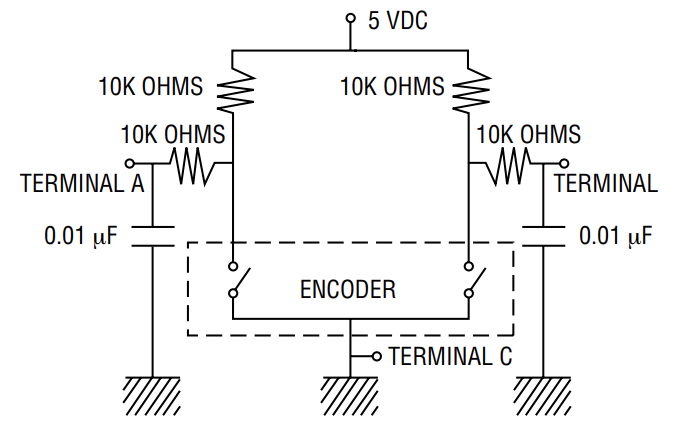
\includegraphics[width=0.65\textwidth]{encoder_karta.png}
    \caption{Schemat filtrów zalecany przez producenta\cite{st:encoder}}
\end{figure}

\begin{figure}[H]
    \centering
    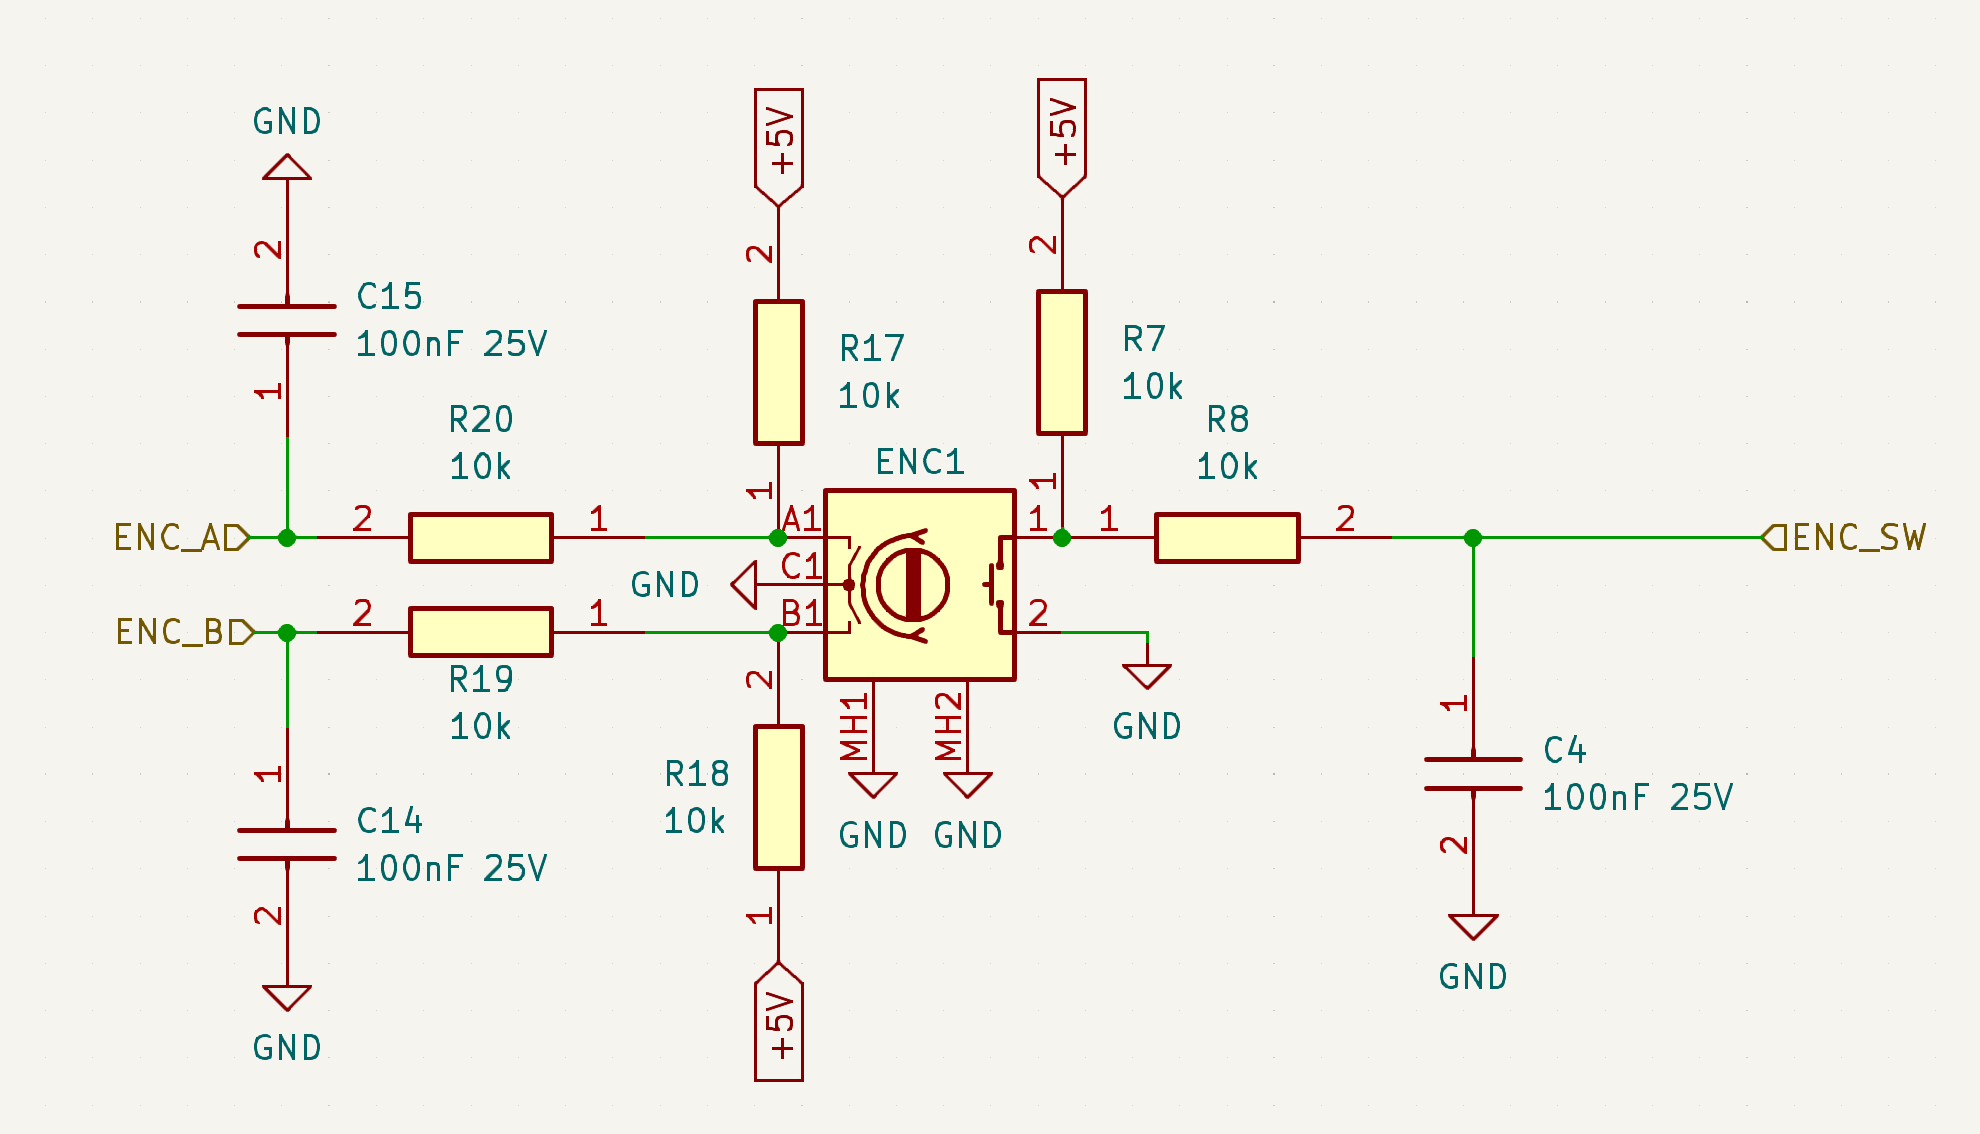
\includegraphics[width=0.8\textwidth]{encoder.png}
    \caption{Gotowy układ encodera}
\end{figure}

\end{document}
